\documentclass[a4paper]{article}

\usepackage[english]{babel}
\usepackage[utf8]{inputenc}
\usepackage{fullpage}
\usepackage{amsmath}
\usepackage{graphicx}
\usepackage[colorinlistoftodos]{todonotes}
\usepackage{hyperref}
\usepackage{amssymb}
% \usepackage{outline} \usepackage{pmgraph} \usepackage[normalem]{ulem}
% \usepackage{graphicx} \usepackage{verbatim}
\usepackage{amssymb} %checklist

\usepackage{wasysym} %checkedbox
\definecolor{mypink1}{rgb}{0.858, 0.188, 0.478}
\definecolor{mypink2}{RGB}{219, 48, 122}
\definecolor{mypink3}{cmyk}{0, 0.7808, 0.4429, 0.1412}
\definecolor{mygray}{gray}{0.4}
 
% \usepackage{enumitem}
% \setlist[description]{style=nextline}

%\usepackage[dvipsnames]{xcolor} 

% \usepackage{minted} % need `-shell-escape' argument for local compile

\title{
    \vspace*{1in}
    
\includegraphics[width=3.25in]{figures/uff-logo.png} \\
    \vspace*{1.2in}
    % \textbf{\huge Weekly Report.}
    \textbf{\huge Report.}
    \vspace{0.2in}\\
    \vspace{0.2in}
}

\author{Luigy Machaca \\
    %\vspace*{0.5in} \\
    \textbf{luigyarcana@id.uff.br} \\
    % \vspace*{1in}
}

\date{\today}


\begin{document}

\maketitle
\setcounter{page}{0}
\thispagestyle{empty}
\newpage


\section{Research Project}
In this project, we will develop a framework system that is a blend that combines object detection, visual object tracking, and one-class classification. This job aims to generate a set of track fragments of each person in the video. Each item is called a tracklet, and a collection of tracklets we called a gallery. Additionally, each of the gallery's tracklets involves the best representative candidate.
\leavevmode\newline
The framework commits a squeezing of the number of queries that will provide to the re-identification algorithm. We will explain these details more later.
\leavevmode\newline
The input of the framework is simple raw video. For this test we use a \textbf{TownCentre} \cite{townCenterDataset} video with the following properties.

\begin{enumerate}
    \item Frames per second = 25 FPS. \label{video:FPS}
    \item Number of frames = 7500 frames. \label{video:number_frames}
    \item Duration of video = 5 minutes 0 seconds \label{video:time}
    \item Resolution of video = 1920 * 1080 \label{video:size}
\end{enumerate}

\subsection{Framework Architecture}

We split this framework into two blocks, where the first part supports the generate tracklets and the second part chooses the best candidate or candidates. It depends on our choice.
\leavevmode\newline
We called the first part how to a cropping module. This module is responsible for generated tracklets. The cropping module receives some arguments that make it a flexible module. We can customize a maximum length of tracklet. We can also decide whether to apply the model in each frame or a specific number of frames.  We can see the next figures [\ref{fig:framework_part1},\ref{fig:framework_part2}].

% \begin{figure}[htp]
\begin{figure}[ht]
    \centering
    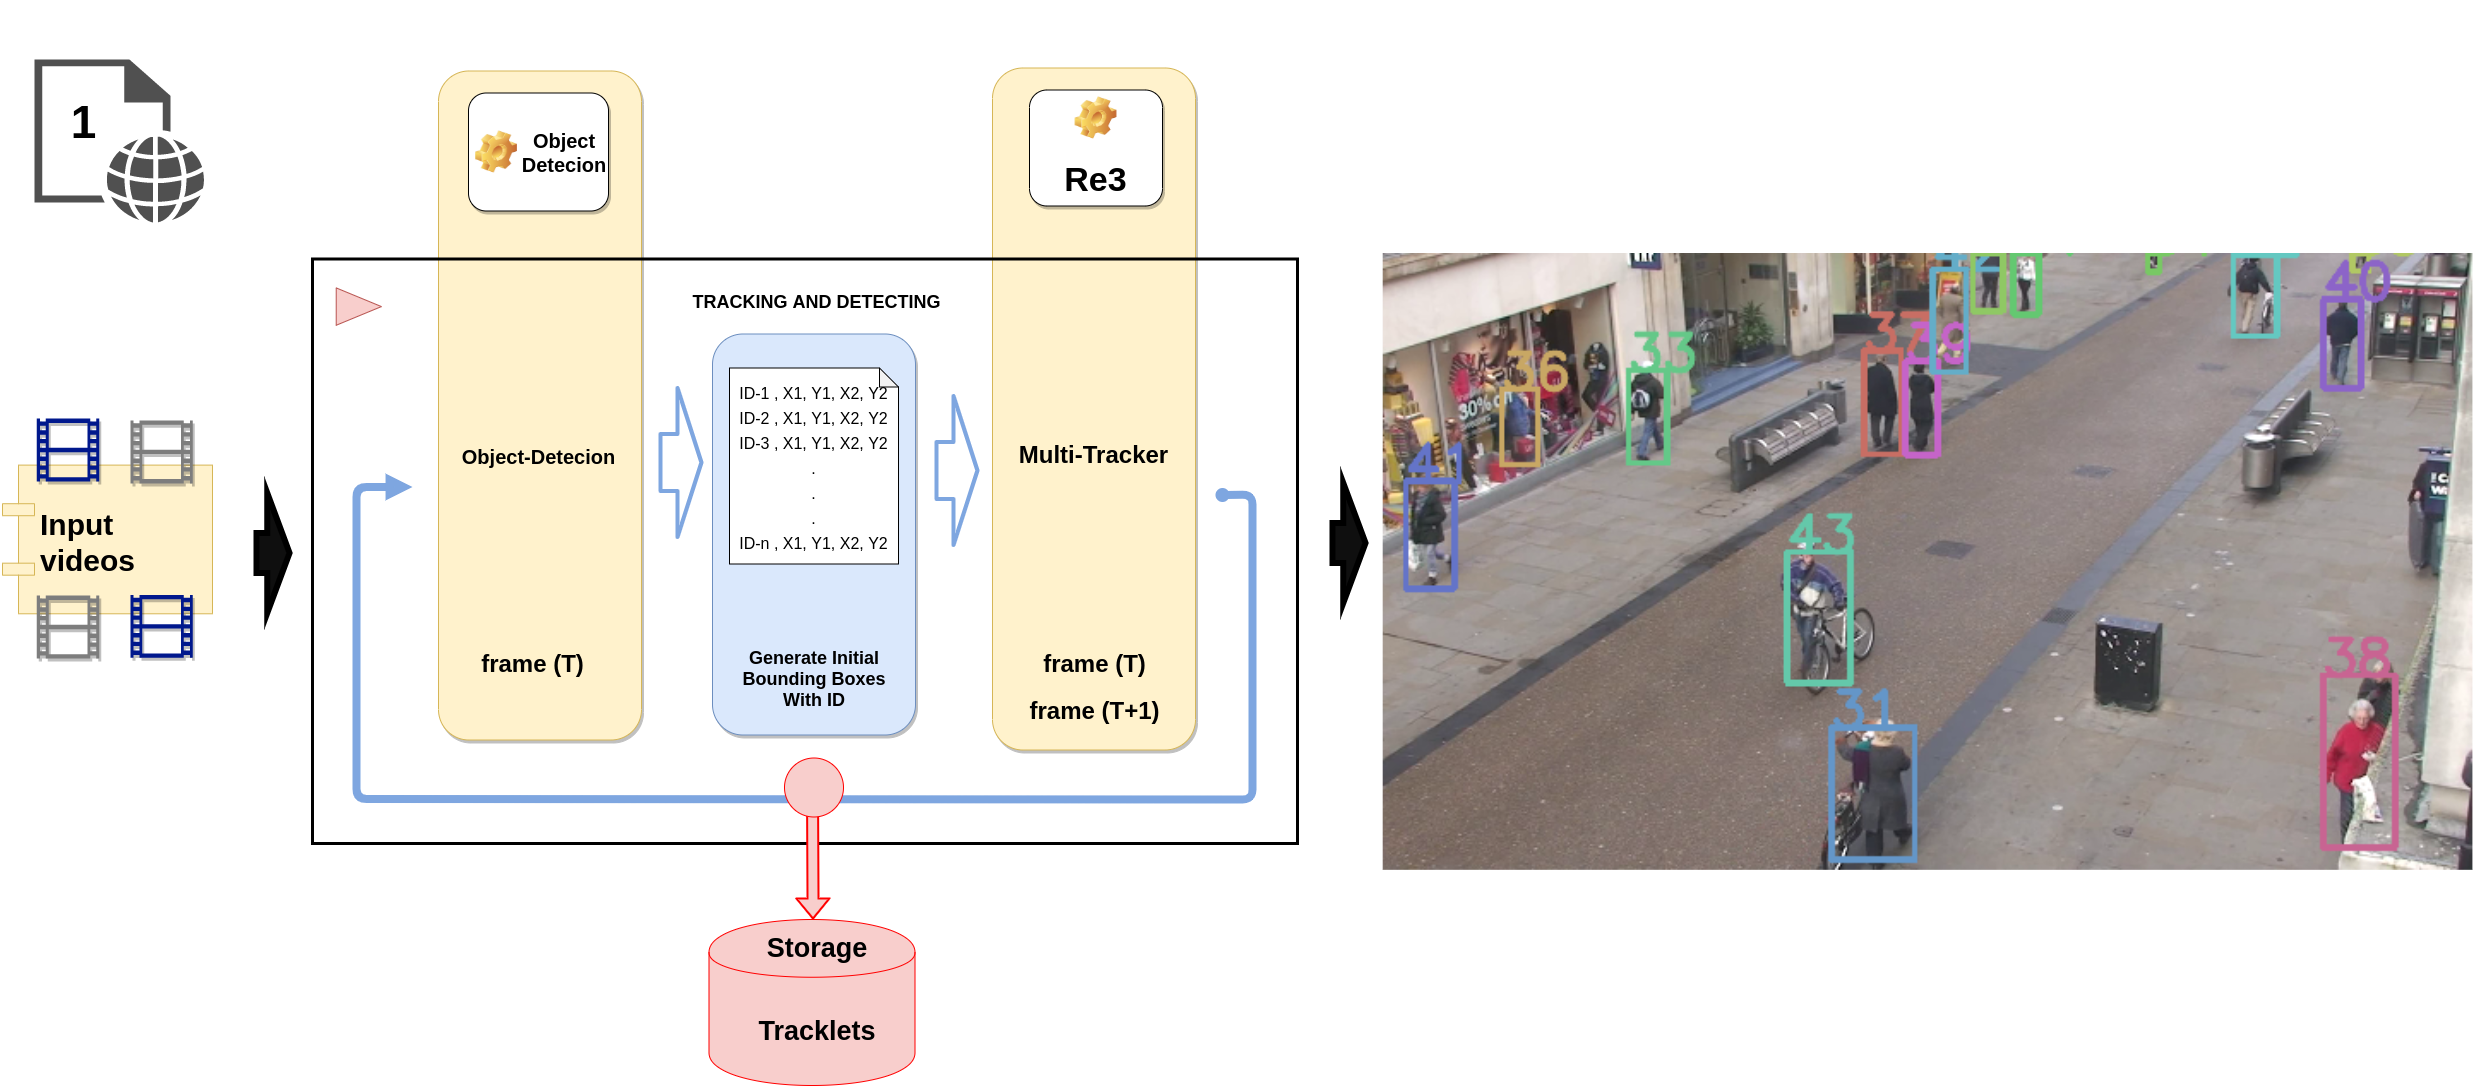
\includegraphics[width=15cm]{imgs/new_model_tesis_2021_part1.png}
    \caption[test framework part 1]{The first part of the framework}
    \label{fig:framework_part1}
\end{figure}\leavevmode\newline

\begin{figure}[ht]
% \begin{figure}[htp]
    \centering
    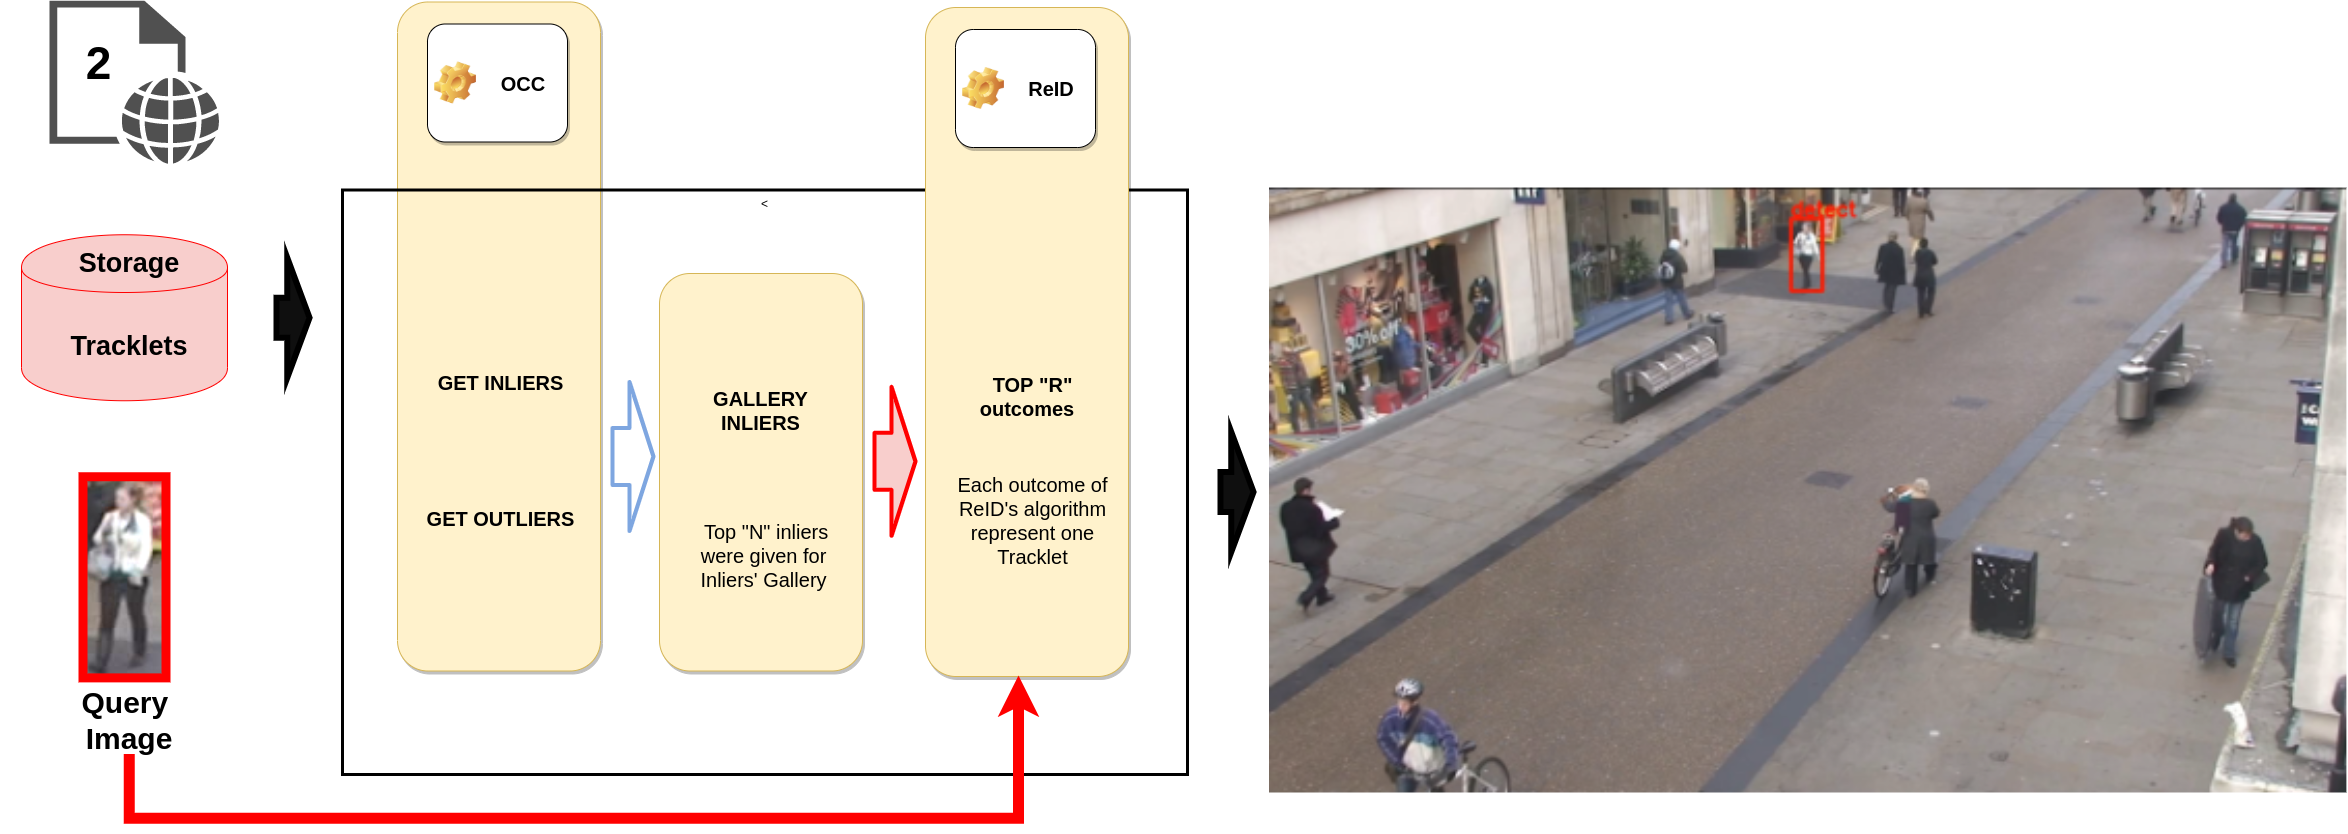
\includegraphics[width=15cm]{imgs/new_model_tesis_2021_part2.png}
    \caption[test framework part 2]{The second part of the framework}
    \label{fig:framework_part2}
\end{figure}\leavevmode\newline


The first module (see figure \ref{fig:framework_part1}) is composed of two algorithms: Object detection and visual object tracking.  We elect  You Only Look Once (YOLO) \cite{YOLO} as an object detection algorithm and Real-Time Recurrent Regression Networks for Visual Tracking of Generic Objects (Re3) \cite{re3} as visual object tracking. 

\leavevmode\newline
We need to remind you that the tracklet is a set of track fragments of each person's video. To generate one tracklet, we need to apply YOLO for the initial coordinates of the track, and the next step will be to use the Re3 in the rest of the tracklet. How to YOLO and Re3 can be detected and track multiple objects at the same time. It allows generating tracklets for each person on the video with 

\leavevmode\newline

In the second module (see figure \ref{fig:framework_part2}), we have two algorithms: Learning Deep Features for One-Class Classification (DOC) \cite{DOC} and An Improved Deep Learning Architecture for Person Re-Identification(ReID) \cite{REID}.  DOC allows us to separate the features representing a class target (person) that other classes (unusual classes), where the main aim to minimize intra-classes and maximize an inter-class distance. In other words, the outcomes of DOC are separated into inliers and outliers. Inliers are likely to have a person and outliers an object or errors that YOLO or Re3 generated. And ReID is designed to address the problem of re-identification for the Query images and our gallery. 

\leavevmode\newline

Creating our gallery, we sorted inliers to deal with their mean where the best inlier is most closely the mean, and we called the inlier representative image. We pick up the inlier representative for each tracklet to support our gallery. And finally, we require a query image and gallery for ReID.

\section{Preliminary results}
We process a TownCenter's video that has a duration of 5 min and has 7'500 frames. For this video, we get 136'099 crops of person. Through these results, we generated 6'972 tracklets where each tracklet has had 20 tracks of a maximum. 
Our gallery for ReID has 6'655 images, and we obtain only the top 10 outcomes. Each of the results represents one tracklet that became easily plot in the video. We find the detection on the next list.


\begin{enumerate}
    \item "inlier" - "time" = 0:00:12
    \item "inlier" - "time" = 0:00:39
    \item "inlier" - "time" = 0:01:10
    \item "inlier" - "time" = 0:03:51
    \item "inlier" - "time" = 0:00:04
    \item "inlier" - "time" = 0:01:06
    \item "inlier" - "time" = 0:03:41
    \item "inlier" - "time" = 0:00:10
    \item "inlier" - "time" = 0:01:09
    \item "inlier" - "time" = 0:03:52
\end{enumerate}


%%%%%%%%%%%%%%%%%%%%%%%%%%%%%%%%%%%%%%%
%%%%%%%%%%%%%%%%%%%%%%%%%%%%%%%%%%%%%%%%%%%%%%%%%%%%%%%%%%%%%%%%%%%%%%%%%%%%%%%%%%%%%%%%%%%%%%%%%%%%%%%%%%%%%%%%%%%%%%%%%%%%%%%%%%%%%%%%%%%%%%%%%%%%%%%%%%%%%%%%%%%%%%%%%%%%%%%%%%%%%%%%%%%%%%%%%%%%%%%%%%%%%%%%%%%%%%%%%%%%%%%%%%%%%%%%%%%%%%%%%%%%%%%%%%%%%%%%%%%%%%%%%%%%%%%%%%%%%%%%%%%%%%%%%%%%%%%%%%%%%%%%%%%%%%%%%%%%%%%%%%%%%%%%%%%%%%%%%%%%%%%%%%%%%%%%%%%%%%%%%%%%%%%%%%%%%%%%%%%%%%%%%%%%%%%%%%%%%%%%%%%%%%%%%%%%%%%%%%%%%%%%%%%%%%%%%%%%%%%%%%%%%%%%%%%%%%%%%%%%%%%%%%%%%%%%%%%%%%%%%%%%%%%%%%%%%%%%%%%%%%%%%%%%%%%%%%%%%%%%%%%%%%%%%%%%%%%%%%%%%%%%%%%%%%%%%%%%%%%%%%%%%%%%%%%%%%%%%%%%%%%%%%%%%%%%%%%%%%%%%%%%%%%%%%%%%%%%%%%%%%%%%%%%%%%%%%%%%%%%%%%%%%%%%%%%%%%%%%%%%%%


% \subsection{Algorithm}
% %\subsection{\textcolor{mygray}{Algorithm}}
% \subsubsection{Re3: Real-Time Recurrent Regression Networks for Visual Tracking of Generic Objects.}
% %\subsubsection{\textcolor{mygray}{Re3: Real-Time Recurrent Regression Networks for Visual Tracking of Generic Objects.}

% %\iffalse
% The tracking pipeline, consists of:
% \begin{itemize}
%     \item convolutional layers to embed the object appearance, 
%     \item recurrent layers to remember appearance and motion information, 
%     \item and a regression layer to output the location for the object. 
% \end{itemize}
% See Figure \ref{fig:re3}

% \begin{figure}[hb]
%     \centering
%     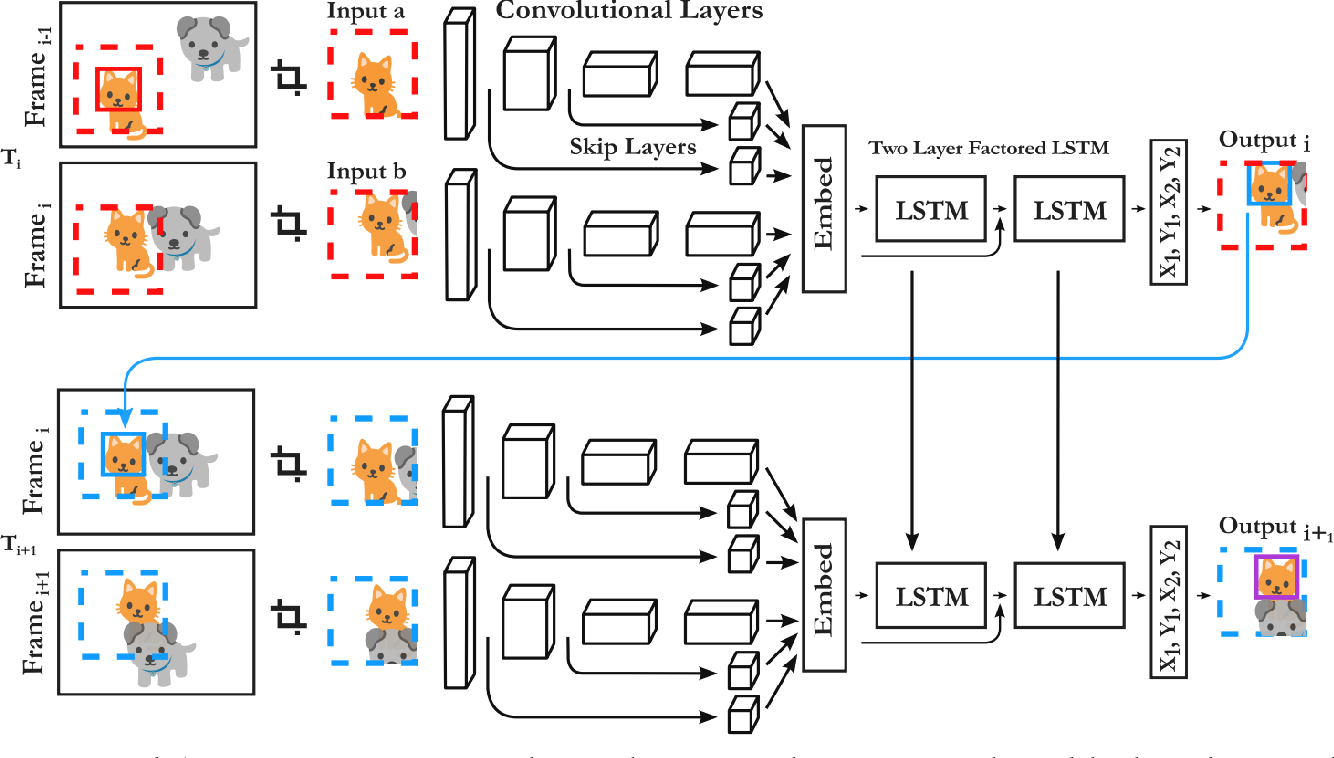
\includegraphics[width=0.6\textwidth]{figures/pipeline-re3.png}
%     \caption{
%             cccccccccc
%     }
%     \label{fig:re3}
%     \medskip
%     \small 
%         \begin{itemize}
%         \item Image crop pairs are fed in at each time step.
%         \item Both crops are centered around the object\'s location in the previous frame 
%         \item and padded to two times the width and height of the object. 
%         \item before every pooling state, to add a skip layer to preserve high-resolution spatial information.
%         \item The weights from the two image streams are shared.
%         \item The output from the convolutional layers feeds into a single fully connected layer and  and LSTM.
%         \item The network predicts the top left and bottom right corners if the new bounding box.  
%         \end{itemize}
% \end{figure}
% %%\fi


% %\subsection{\textcolor{mygray}{Dataset}}
% \subsection{Dataset}

% %\iffalse
% The VOT challenges provide the visual tracking community with a precisely defined and repeatable way of comparing short-term trackers as well as a common platform for discussing the evaluation and advancements made in the field of visual tracking.
% \cite{VOT2014} \cite{VOT2016}
% \begin{itemize}
%     \item VOT 2014
%     \item VOT 2016
% \end{itemize}
% %\fi



%\iffalse
%\subsection{Doxygen}
%Doxygen is a tool for documenting code that is compatible with Python. Doxygen provides most of the functions, but it is also a bit complicated. Because of the amount of work he does, he does it at a very fast speed.
%\begin{itemize}
%    \item Written and compiled in C ++, this is the fastest of the tools by far.
%    \item You can generate documentation in several ways, not just in HTML.
%    \item Supports Markdown and documentation pages
%    \item You can easily see the source directly from the documentation.
%    \item Diagrams with the structure of your code. 
%\end{itemize}
%\fi


% \section{Progress}



%\iffalse
%\begin{description}
%\item [$\checkmark$ \textcolor{mygray}{Step 1}] Research, install and test Docker \& Nvidia on remote PC.} 
%\item[$\checkmark$ \textcolor{mygray}{Step 2}] \textcolor{mygray}{ Building instances for Nvidia-docker.}
%\item[$\checkmark$ \textcolor{mygray}{Step 3}] \textcolor{mygray}{Fixed problems for network connection and port of remote PC  with a VPN.}
%\item[$\checkmark$ \textcolor{mygray}{Step 4}] \textcolor{mygray}{Replicate results and test of Re3 \cite{re3} on Docker container.}
%\item[$\checkmark$ \textcolor{mygray}{Step 5}] \textcolor{mygray}{Fixed problems with CUDA version and requirements of Re3.}
%\item[$\checkmark$ Step 6] \textbf{Analyzing} Copacabana surveillance videos.
%\item[$\checkmark$ Step 7] Copacabana videos has been \textbf{spitting} frame per frame. [opencv-python]
%\item[$\checkmark$ Step 8] The code re3 is being \textbf{documented}. [Doxygen]
%\end{description}
%\fi

% \begin{description}
% \item [$\checkmark$ Step 1] Research, install and test Docker \& Nvidia on remote PC.
% \item[$\checkmark$ Step 2] Building instances for Nvidia-docker.
% \item[$\checkmark$ Step 3] Fixed problems for network connection and port of remote PC  with a VPN.
% \item[$\checkmark$ Step 4] Replicate results and test of Re3 \cite{re3} on Docker container.
% \item[$\checkmark$ Step 5] Fixed problems with CUDA version and requirements of Re3.
% \item[$\checkmark$ Step 6] \textbf{Analyzing} Copacabana surveillance videos.
% \item[$\checkmark$ Step 7] Copacabana videos has been \textbf{spitting} frame per frame. [opencv-python]
% %\item[$\checkmark$ Step 8] The code re3 is being \textbf{documented}. [Doxygen]
% \item[$\square$ Step 8] \textbf{Testing} Re3 with multiple people.
% \item[$\square$ Step 10] Create a \textbf{Pipeline}, where Re3 is going to be a module of \textit{Framework}.
% %\item[$\square$ Step 11] \textbf{Training} with data set.
 


% \section{Plan}

% \begin{tabular}{rl}
% 	\textbf{Objective:} & Framework tracking multiple people \\
%     %\textbf{Deadline:} & 22 may 
% \end{tabular}


%     \begin{description}
%         %\item[\normalfont 2019.02.07---2019.05.14] Do something.
%         %\item[\normalfont 2019.05.15---2019.05.22] Do something else.
%         %\item[\normalfont 2019.05.23---2019.05.31] Do a lot lot lot lot lot lot lot lot lot lot lot lot of things.
%         \item[$\square$ Step 11] move all project to NIXos
%         \item[$\square$ Step 12] improve module \textbf{tracking}, where algorithm      \textbf{YOLO} is going to be a sub-module of \textit{tracking}.
%         \item[$\square$ Step 13]  
%     \end{description}
% \end{description}




% If you don't cite any references, please comment the following two lines
% \newpage
\nocite{*}
\bibliographystyle{ieee}
\bibliography{ref.bib}





\end{document}

